\subsection*{engineering}
i assembled a simple ring modulator mockup in ltspice, which served to
illustrate the basic mechanics of making one. the difficulties in using a ring
modulator for direct upconversion is the input inductance and frequency -- the
modulating signal is coupled in through a transformer, which must operate both
at \rf and \ifreq.

fortunately, interchanging \rf and \ifreq leads to a still-working modulator! a
schematic is given in figure \ref{fig:ring-mod-spice}.

\begin{figure}[H]
	\centering
	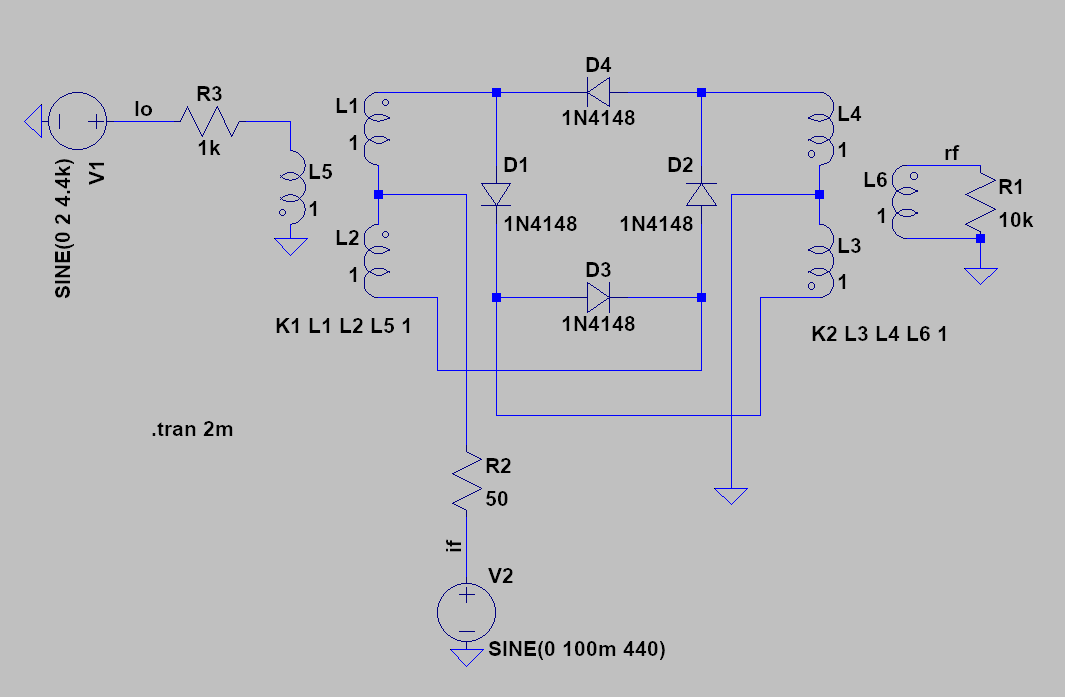
\includegraphics[width=.9\textwidth]{ring-mod-spice.png}
	\caption{ring modulator ltspice prototype}
	\label{fig:ring-mod-spice}
\end{figure}

the next step is to manage a \ssb transmitter. the basic process for \ssb
modulation is to modulate an in-phase \amp quadrature signal with the original
signal \amp its hilbert transform, respectively, as described in
\autocite{matlab-ssb}. this, however, requires a hilbert transformer\ldots\
which is apparently often implemented approximately with a filter, and in the
digital realm!

i decided to fiddle with \ssb modulation in octave to see if i could come up
with a good way to do it, starting with basic info about the behavior of the
hilbert transform. the code may be found in
\localfile{../work/am-mod/code/ssb.m}. initial conclusions were that \ssb is
mathematically feasible, but generation of the appropriate input signal was the
sticking point.

actual architectures for creating a quadrature phase shifter are described in
\autocite{wideband-shifter} and \autocite{audio-shifter}. these were used as
inspiration for the rest of the work here. \autocite{wideband-shifter}
describes an \textsc{rc-cr} network employed by hartley to produce the
appropriate signals, consisting of a high-pass and a low-pass filter, but the
difficulty with this method is its lack of bandwidth and variable gain with
frequency -- no good.
